\chapter{Embedded Development}\label{chap:embedded}

During a meeting with the project's client, the possibility of obtaining a prototype sub-threshold device from ARM was briefly discussed. However, this was quickly dismissed as it was still in development, meaning there are only a few built versions and these may not be in a suitable state for active development. As such, it was decided that the constrained conditions would, instead, need to be emulated. Emulation proved to be useful, as it allowed the team to use limited conditions when developing and testing the system, but still able to use larger systems such as serial communication for the purposes of debugging.

\section{Processor Emulation}

\namedsubsection{ARM Cortex M0 Processor \label{sec:cortex}}{Pasat}

This section discusses one of the main requirements and one of the essential aspects of the project: using ARM's Cortex M0 processor. This processor is a member of the Cortex-M family and offers a great tradeoff between costs and performance/functionality. It has been designed in order to allow intelligent compromises in terms of power usage, computational power and in the simplicity of the design. It implements a simplified version of the Advanced Microcontroller Bus Architecture (AMBA), the AMBA-Lite Bus, which allows connection to different peripherals. In this way, the Cortex-M0 generally acts as the master device and the peripherals act as slaves. In figure \ref{fig:cortexm0ds}, the schematic for the processor can be seen.\\
\begin{figure}
\centering
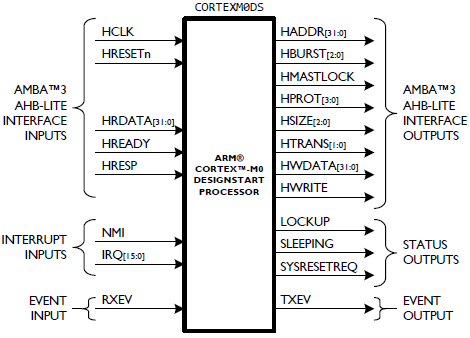
\includegraphics[scale=0.7]{figures/cortexm0ds_schematic.PNG}
\caption{Cortex M0DS schematic \cite{armdesignstart}} \label{fig:cortexm0ds}
\end{figure}
\clearpage

\begin{figure}
\centering
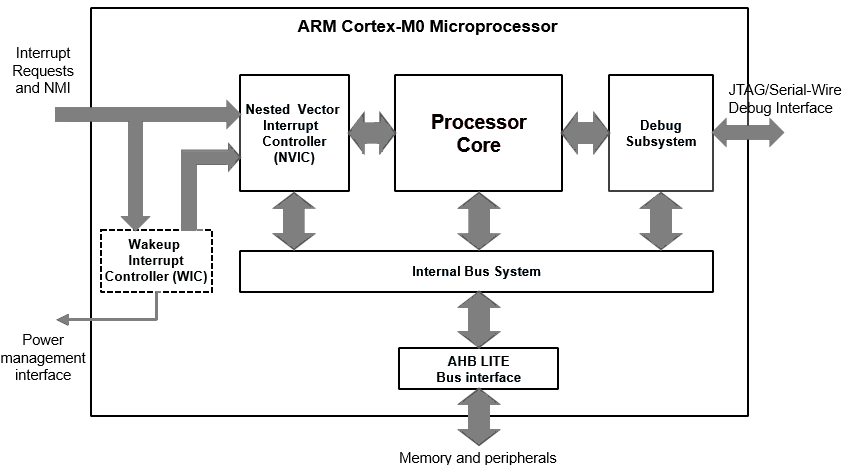
\includegraphics[scale=0.7]{figures/arm_cortexm0_microprocessor.PNG}
\caption{Cortex-M0 Block Diagram \cite{armdesignstart}} \label{fig:cortex_block}
\end{figure}

The Cortex M0 has a 32-bit reduced instruction set computing (RISC) processor. It uses the ARMv6-M(Microcontroller), which is a subset of the ARMv7-M profile but includes fewer instructions. The Cortex M0 is based on a Von-Neumann architecture, having both data and instructions share a single bus interface. It provides a Debug Extension that includes some architectural extensions to support debugging. The ARMv6-M offers support for 56 instructions as a subset of  Thumb-1(16-bit) and Thumb-2(16/32b-bit) which are present in the ARMv6T2. The Cortex M0 block diagram can be seen above in figure \ref{fig:cortex_block}. 

The Processor Core contains the internal registers, data path, ALU and control logics. The Cortex M0 has a three-stage pipeline: fetch, decode and exection and includes the 32-bit registers for general and special usages. The Cortex M0+ has only a two-stage pipeline to reduce the power usage.

The Nested Vectored Interrupt Controller (NVIC) handles up to 32 interrupts request signals and one NMI (Non-Maskable Interrupt). It also fulfils tasks such as comparing priorities between  interrupt requests and the current priority level. 

The Bus system contains the internal bus system, the data path in the processor core and the AHB LITE interface unit which is an on-chip bus protocol which enables some features required for high-performance, high clock frequency systems. 

The Debug system handles the program breakpoints, debugging control and the data watchpoints. This can put the processor in a  static state in order for the programmer to evaluate and analyse the status of the processor in that specific moment.

The Wakeup Interrupt Controller (WIC) is important for this project because it is used in low-power applications. The microcontroller can be set to enter sleep mode by turning off most of its components. If a interrupt request is sent, this component can inform the unit that handles the power management to power up the system.

\subsubsection{Limitations \label{sec:cortex-limitations}}

One of the major challenges which was encountered in the use of the Cortex M0 is the lack of hardware division or floating point unit. To account for this, there are software libraries which perform these operations however, they can take quite a large number of cycles to perform and hence would be impractical on a constrained system.

Since the Cortex M0 is such a low-power, lost-cost device, it comes with its limitations. The device only offers 32kB on-chip flash programming memory and only 8kB SRAM. Basic applications have been developed for this processor, but in order to allow the implementation of a more complex program, such as exercise recognition, the code and libraries need to be very well optimised. All the unnecessary functionalities available in libraries must be disposed in order to save memory on this constrained system.
\namedsubsection{FPGA}{Pasat}

An Field-Programmable Gate Array (FPGA) is a semiconductor device which is has a matrix of Configurable Logic Blocks (CLB) connected through programmable interconnects. One main advantage of the FPGA is that it can be preprogrammed after they are manufactured in order to fit desired functionalities and requirements. Interesting projects have also been realized with this processor on a FPGA, such as advanced real traffic light controller \cite{traffic_light}.

Typically, the FPGA differs great from the conventional microcontroller; the microcontroller has the chip already designed. The programmer simply writes the software in C or C++, then it is compiled into a hex file that is loaded on the microcontroller. The program is stored in the flash memory until is is replaced or erased.

FPGAs are different in this sense. The circuit is completely designed by the programmer. The processor must be created and can be as simple as an and gate or can be our Cortex M0+. HDL is used to write the design, which is then synthesized into a bit file which configures the FPGA. One small problem with this is the fact that it stores the configuration in the RAM, so once the power is gone, the configuration is lost.

The board used for this project is the Xilinx Digilent Nexys4, which can be seen in figure \ref{fig:nexys4}. It is based on the Artix-7 which has a low power consumption and cost \cite{cortexm0onnexys4}. Implementations were also successful on low end FPGAs. This board was chosen because it is a large, high-capacity FPGA board that would be sufficient for our project. Another reason is the fact that is has several built in peripherals, such as accelerometer, which would be useful for the exercise detection. 

\begin{figure}
\centering
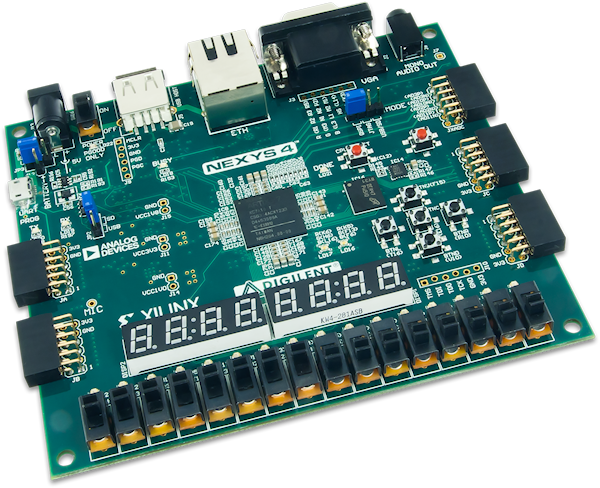
\includegraphics[scale=0.7]{figures/nexys4.PNG}
\caption{Xilinx Digilent Nexys4 \label{fig:nexys4}}
\end{figure}

\namedsubsection{mBed}{Gupta}

mBed is a platform which implements ARM 32-bit processors within micro-controllers which is primarily developed by ARM. They are of the DIP form factor with 40 pins. It features an online SDK allowing for the development of projects online. It permits code to be written online as well as compiled into a binary compatible with the board being used. This binary can then be downloaded removing the pre-requisite of having the ARM toolchain available locally. The manner of uploading to the mBed is relatively straight forward with the presence of the mBed interface. \cite{mbed_website}\todo{Try expanding on this section}

This interface exposes a Mass Storage device to the host computer via a USB connection allowing for binaries to be uploaded in a drag and drop manner. The interface is also connected with the target chip using a JTAG connection allowing for it to program its flash memory. When the reset button is pressed, the interface checks the storage for the newest binary file and, should it not be programmed within the device already, will program the binary provided into the flash memory of the chip. \cite{mbed_website}\todo{Try expanding this section as well}

\subsubsection{Why the mBed}

When \todo{Need a better name for this subsection?} initially looking at various ways to emulate the sub-threshold version of the ARM Cortex M0, using an existing non sub-threshold version of the ARM Cortex M0 was considered. This involved searching for some form of micro-controller or device which would allow for programming of the processor. This lead to the mBed family which appeared easy to program and use featuring ARM processors. Within the mBed family of micro-controllers, the LPC11U24 model uses an ARM Cortex M0 as its processor.

An important factor for the device is being able to communicate with other devices using various communication protocols. Fortunately, multiple pins are broken out on the mBed which allow for flexibility in choice, in particular there are 2 SPI, 1 I2C, and 1 Serial interfaces available simultaneously upon the mBed. \cite{mbed_website} 

For obtaining data from the sensor, it is most likely to use I2C or One-Wire communication, should it be I2C, the mBed would work well. It also allows for the Serial pins to be interfaced with the host PC allowing for debugging information to be transmitted to the host PC. 

The requirements for this project require the processor to be emulate the sub-threshold version which operates with a system clock in the range of a few hundred kHz to a few MHz. This would require a clock in the micro-controller which can operate at these frequencies and also be able to be set as the system clock.

The device typically runs at 48MHz using its Internal RC oscillator (IRC) as its system clock. However, it also has the ability to switch its system clock to be sourced from the internal Watchdog oscillator instead. 

This oscillator consists of two parts, an oscillator function which generates an analog clock (\verb|Fclkana|) as well as a divisor (\verb|DIVSEL|) which is used to divide the analog clock to the required output frequency (\verb|wdt_osc_clk|). The output frequency can be calculated using Equation~\ref{eq:wdt_osc_clk} and is within the range $ 9.4 $ kHz $ \leq \verb|wdt_osc_clk| \leq 2.3 $ MHz. \cite{mbed_datasheet}

\begin{equation}
	\label{eq:wdt_osc_clk}
	\verb|wdt_osc_clk| = \frac{Fclkana}{2 * (1 + DIVSEL)}
\end{equation}

Some concerns were made realising that the Watchdog oscillator has an error margin of $\pm 40\%$ for the frequency of Fclkana. In a meeting with the client, it was decided to carry forward with the device while paying attention to this margin and analysing the impact of it upon the project.
\namedsection{Initial Design}{Gupta}

The hardware side of this project requires the ARM Cortex M0 processor to obtain the sensor data to classify with the model. The classification then needs to be made visible so a user can see whether they are doing exercise or not, this can be done simply with something such as an LED. During development, it is also useful for debug information to be extracted so it is possible to diagnose issues that may arise as well as test various parts of the system ensuring that they work as expected. 

Figure~\ref{fig:hardware_schematic_development} shows the block diagram for the hardware part of the project whilst still developing and Figure~\ref{fig:hardware_schematic_final} shows the block diagram for the target final system.

\begin{figure}[!hb]
	\centering
	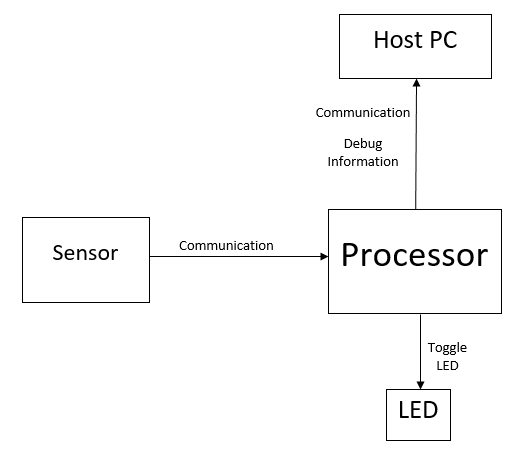
\includegraphics{hardware-schematics-development.pdf}
	\caption{Hardware Block Diagram - Development}
	\label{fig:hardware_schematic_development}
\end{figure}

\begin{figure}
	\centering
	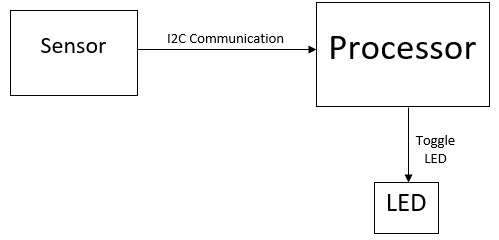
\includegraphics{hardware-schematics-final.pdf}
	\caption{Hardware Block Diagram - Final}
	\label{fig:hardware_schematic_final}
\end{figure}

\namedsection{FPGA}{Pasat}

The FPGA was initially designed to have a Cortex-M0\_DS processor, a block of memory with a program that fetches constants from that block at regular intervals, a reset and a pattern detector attached to the bus so when a specific pattern appears on the data bus, the LED turns on and when another patters appears it will turn off. The Cortex-M0\_DS  includes only the processor and a non-synthesisable testbench. Other parts will need to be implemented in order to create a synthesisable system: a software executable image, a system clock, a detector module for the command LED and a reset synchroniser. This section will be divided into: software development and simulation, system implementation and functional simulation. All of these sections will be discussed in detail in what follows.

\begin{figure}
	\centering
	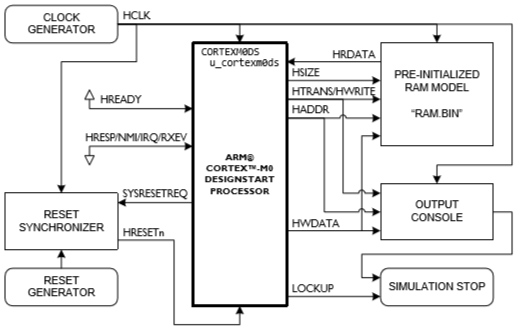
\includegraphics[scale=0.7]{figures/test_bench_schematic.PNG}
	\caption{Cortex M0 test bench schematic} \label{fig:test_bench}
\end{figure}

Through ARM, access was obtained to a fixed configuration of the Cortex-M0 Processor known as Cortex-M0 DesignStart \cite{armdesignstart}. This simplified version offers us access to a Verilog version of the Cortex-M0 under the form of an obfuscated and preconfigured netlist, but it can be synthesised. This package also includes a test-bench which allows for simulation of the Cortex-M0 DesignStart module connected to a memory model and a clock and reset generator. It also includes a basic C \verb|helloworld.c| program. The schematic for the test-bench can be seen in figure \ref{fig:test_bench} and it connects the CORTEXM0DS to a memory model, a clock and a reset generators.

ModelSim was used for running the test-bench, which is a tool that offers the possibility of simulating hardware description languages such as Verilog and VHDL.  A memory image, provided within the DesignStart package, is used for the \verb|helloworld.c| program, which is used by the test-bench to write a message to the simulator's console and after that end the simulation. 

Also, access was given to the CM0DS example design kit which contains various AHB-Lite peripherals and infrastructure components, useful to create complete systems. Before implementing the actual algorithm on the FPGA, a more basic simulation needs to be conducted on the platform to assure that it is compatible with the specific FPGA used. Next, the analysis of the sensors used for our project will be discussed. 


\subsection{Software Development and Simulation}
In this section, a software program that will verify the memory fetches of some predefined constants. The program used for this will be the IDE ARM Keil $\mu$Vision which allows quick and easy building of projects.

To start, a new project must be created in $\mu$Vision. Next, the device must be selected device database so ARM-ARM Cortex M0 plus-ARMCM0P is selected which can be seen in figure \ref{fig:armcm0p}.

\begin{figure}
\centering
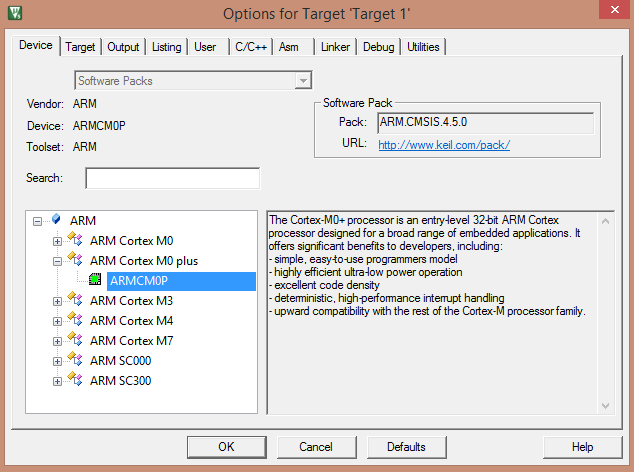
\includegraphics[scale=0.7]{figures/armcm0p.PNG}
\caption{Selection of the Cortex M0+ for the μVision project} 
\label{fig:armcm0p}
\end{figure}

After this is selected, the options menu is accessed for this device. Next, the target options need to be accessed and the following modification need to be made:

\begin{itemize}

\item {Under Target section, the Read/Write Memory Areas, RAM1 starts at 0x0 and has the size of 0x400000 (this setting is used to create a linker scatter file. Another requirement for this is the having the Use Memory Layout from Target Dialog enabled in the Linker section)}

\item {Output section, the Debug Information and Browse Information sections need to be ticked(this defines the resulting output files from the tool chain and allows the user programs to be started after the building process is complete)}

\item {Under Listing section, all the default selected features stay the same(here all the listing files generated by the tool chain are specified)}

\item {Under User section, in Run\#1:"fromelf -cvf code.axf --vhx --32x1 -o code.hex" and Run\#2:"fromelf -cvf code.axf -o disasm.txt" in Run User Programs After Build/Rebuild those code lines are inserted in order to create a .axf file from the .hex file}

\item {Under C/C++ section, the One ELF Section per Function is unticked and the Warnings are set to "unspecified" (here C/C++ specific tool options are set)}

\item {Under Asm section, all the settings are kept to default also(this allows the setting of specific Assembler tool options)}

\item {Under Linker section, the R/W Base entry is deleted and only the R/O Base: 0x00000000 remains(linker settings are required in order to configure the physical memory location of the target). The location of memory classes and sections is defined here.}

\item {Under Debug section, the default settings for µVision4 Debugger stay the same}

\item {Under Utilities, the Use Target Driver for Flash Programming in the Configure Flash Menu Command is left checked.}

\end{itemize}

\begin{lstlisting}[caption={Reset Handler},label={lst:reset-handler}]
Reset_Handler	PROC
		GLOBAL Reset_Handler
		ENTRY

AGAIN		LDR	R1, =0x50000000		;Write to LED with value 0x55
		LDR	R0, =0x55
		STR	R0, [R1]


		LDR	R0, =0x2FFFFF		;Delay
Loop		SUBS	R0,R0,#1
		BNE Loop

		LDR	R1, =0x50000000		;Write to LED with value 0xAA
		LDR	R0, =0xAA
		STR	R0, [R1]

		LDR	R0, =0x2FFFFF		;Delay
Loop1		SUBS	R0,R0,#1
		BNE Loop1
\end{lstlisting}

After all of these steps have been done, it is now time to add the assembly file provided by ARM, the \verb|cm0dasm.s| to the source. Taking a look at the reset handler, which can be seen in \ref{lst:reset-handler}, it turns on half of the 8-bit LEDs (for example 0, 2, 4 ,6), sets up a counter and uses it for a short time delay, then turns on the other half and delays another period.

After the successful building, the code.hex should be created and converted into a .axf because it was set in the User section. The .axf file needs to be converted to a .bin in order to program the FPGA. The MDK/Keil offers a tool called "fromelf" which can do this conversion. It is called as shown in listing \ref{lst:elf-to-bin}:

\begin{lstlisting}[caption={Creating a bin file from ELF Format},label={lst:elf-to-bin}]
fromelf --bin --o code.bin code.axf
\end{lstlisting}

This can be used to program the FPGA. Now, the implementation of the Cortex-M0 will be discussed.

\subsection{System Implementation}

The simulated ARM Cortex-M0 processor includes the AHB-Lite system bus and two AHB peripherals: the program memory (which will be implemented using on-chip memory blocks) and a simple LED peripheral. Some of the steps are similar for implementing the Cortex M0 on a older FPGA~\cite{implementationcortexm0onnexys2}, but since different modules and software are required, some of the same steps may not apply.

The software used for this implementation was Vivado Design Suite produced by Xilinx. This is used for synthesis and analysis of HDL designs. It is a improved version of the Xilinx ISE which also allows features such as system on a chip development and a high-level synthesis. 

The Cortex-M0 DesignStart will be used, which is a simplified version of the industry Cortex-M0 processor, but has some features reduced which are not essential for this project such as the number of available interrupts (from 32 to 16). Two verilog files are included in this pack:  \verb|cortexm0ds_logic.v| and \verb|CORTEM0DS.v|. The \verb|cortexm0ds_logic.v| contains the Cortex-M0 DesignStart processor logic level Verilog file, while the CORTEXM0DS.v includes the Cortex-M0 DesignStart processor macro cell level.

On-chip memory block are used in order to implement the program memory in SoC, for example the Block RAM (BRAM) which is present on this FPGA. The program image needs to be merged into the hardware design during synthesis to load the program on the on-chip memory of the FPGA.

Now, in order to implement the Cortex M0 on the FPGA, more than just the ARM DesignStart Verilog codes are necessary. The ARM Cortex-M System Design Kit (CMSDK) contains a set of \verb|AMBA|, \verb|AHB| and \verb|APB| components and examples for various Cortex-M systems processors, including the Cortex-M0. The  Verilog file  used from this package in order to reproduce the desired experiment will be discussed.

The \verb|AHBDCD.v| contains the code for the address decoder of the \verb|AHB| bus. This uses a Multi-layer bus architecture having only one \verb|AHB| master on each of the input layers and one \verb|AHB| slave on each of the outputs, the entire system address decoding can be done within the decoder section. 

The \verb|AHBMUX.v| contains the code for the slave multiplexor of the \verb|AHB| bus. This uses parameters in order to specify the slave port usage in order for the synthesis process to no generate extra logic which is not necessary for the project. The slave to master multiplexer controls the response signals and read data routing from the bus slaves to the bus masters. The address decoder presented earlier is used to determine the currently selected slave and generates the \verb|HSEL| signal to the \verb|AHB| slaves and slave multiplexer. The multiplexer creates the connection between the slave outputs and the inputs of the bus masters. 

\begin{figure}
\centering
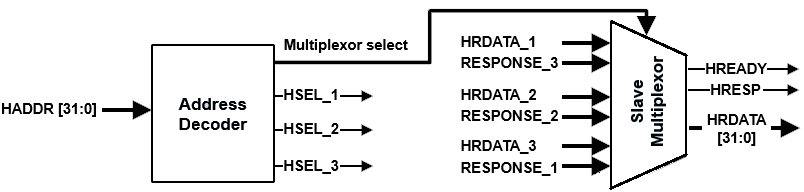
\includegraphics[scale=0.7]{figures/decoder_and_multiplexer.PNG}
\caption{Address Decoder and Slave Multiplexor\cite{ahblite} } 
\label{fig:decoder_multiplexer}
\end{figure}

Figure \ref{fig:decoder_multiplexer} shows how two Address Decoder and Slave Multiplexor can be seen. The \verb|HADRR|[0:31] signal sends the read data from multiplexer to master \cite{ahblite}. The \verb|HREADY| signal goes from the multiplexor to the master and slaves and when it is set to HIGH, it indicates that the previous transfer has been completed. The \verb|HRESP| signal transfers the response signal from multiplexor to master. Each of the slaves has its own select signal \verb|HSEL| which indicates the current transfer intended for that specific slave. Before being able to respond to the current transfer, the status of \verb|HREADY| must be known in order to ensure that the previous transfer has been completed. 

The \verb|AHB2BRAM.v| contains the on-chip memory peripheral (BRAM) 
which is a configurable memory module that gives access to a variety of BRAM Interface Controllers. This is used for the program memory of the processor.

The \verb|AHB2LED.v| contains the LED peripheral module. Selected LED will light up when a specific generated patters will be detected and will turn off when another pattern is detected.

The \verb|AHBLITE_SYS.v| contains the top-level module. The AHB-Lite is a subset of the full \verb|AHB| specification which is used in designs where there is no more than one bus master used. This simplifies the \verb|AHB| specification because it removes the unnecessary protocol used for more bus masters.

The \verb|ARMSOC_s6.ucf| file is the user constraint file which creates the connection between the assigned nets and FPGA pins.

All of these files files need to be added to a Vivado project in order to create and download the bitstream file to the FPGA. A new project was created, specifying that it is a RTL project. A mixed implementation setting between Verilog/VHDL will be required for this project. The processor is described in Verilog while the additional modules are in VHDL. Next, in the list of Xilinx parts, the XC7A100T-1CSG324C needs to be selected because this is the part name for the Nexys4 board. 

\begin{figure}
\centering
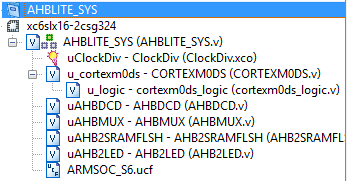
\includegraphics[scale=0.7]{figures/AHBLITE_SYS_modules_ISE_schematic.PNG}
\caption{AHB Lite top-module } 
\label{fig:ahblite_sys}
\end{figure}

After the project is created, the \verb|AHBALITE_SYS.v| is set as a top module since this creates the connection between all the components. This can be seen in \ref{fig:ahblite_sys}. Because this is a Nexys4 board and the Clock Divider supplied in the package are not compatible due to the fact that it requires a Spartan 6 Series processor, a new IP needed to be created for this specific FPGA. In order to add this we need to go to Source-New Source-IP CORE(Generator and Architecture Wizard)-Clocking-Clocking Wizard. This is going to generate a system clock at 10MHz from the board's 50MHz external oscillator. In figure \ref{fig:clock}, the Input Clock Frequency is set 50 MHz and the Output Frequency to 10 MHz and it is named "uClockDiv".

\begin{figure}
\centering
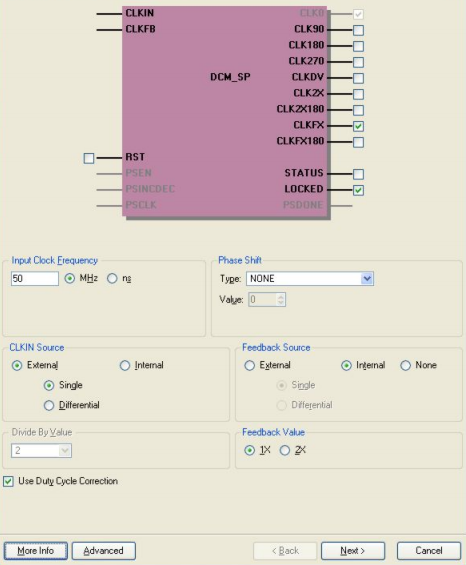
\includegraphics[scale=0.7]{figures/clock_creation.PNG}
\caption{Clocking Wizard settings } 
\label{fig:clock}
\end{figure}

Since the user constraint file supplied is meant to be used to a Spartan 6 Series FPGA board, the user constraint file needed modifications in order to fit the Artix-7 FPGA. The UCF can be seen in appendix \ref{ch:ucffile}. After this, the top module of the simulation can be implemented and translated int o a .bit file which is used to program the FPGA.

\subsection{Functional Simulation}
Due to some unplanned delays in acquiring certain documentation, delays in obtaining licenses for the various software used, and difficulties encountered during the creation of a proper .bit file, a full functional simulation was not properly conducted. A basic simulation of the Cortex M0 was presented in section~\ref{sec:cortex}.  The functional simulation of the system verifies if the signal in \verb|HRDATA| are the ones expected and if it works as expected. This is accessed by going to Design-View:Simulation. If a complete functional would have been performed, a run-time simulation needs to also be performed. On-chip debugging tools such as ChipScope are required in order to perform this sort of simulation. Inside the analysis, these AHB signals need to be evaluated to see if they work correspondingly: 
\begin{itemize}
\item \verb|HADDR|[31:0] 
\item \verb|HWDATA|[31:0]
\item \verb|HRDATA|[31:0]
\item \verb|HWRITE|
\item \verb|HREADY|
\item \verb|HSIZE|[2:0]
\item \verb|HTRANS|[1:0]
\item \verb|HRESP|
\end{itemize}

\namedsection{Sensor}{Gupta}

The sensor chosen, Xadow IMU 6DOF which uses the MPU6050 chip, allowed for a great deal of versatility by means of configuring the various registers contained within the MPU6050. This allowed for the option to use what was required by the sensor and nothing else, thus helping to minimise the power consumption of the device where possible. \cite{sensor_specs}

The primary usage of the sensor to the project, are the 3-axis accelerometer and gyroscope which can be used to measure the acceleration and angular velocity upon the foot. The data collected can be extracted from the sensor using I2C communication. 

When reading values from the sensor, the raw value is received. This is a value in the range -32768 to 32767 which then needs to be translated to an actual value. The relationship between the raw value and the actual value is dependant on the sensitivity configured for the accelerometer or gyroscope. The typical values for the sensitivity are $\pm 2g$ and $\pm 250~\degree / sec$ respectively. The sensitivity can be considered the maximum value that the sensor will provide, ie the sensitivity values are also the values at either end of the raw value range. This leaves a linear scale in between allowing for easy calculation of the reading given the sensitivity and the raw value. For example, a range of $\pm 2g$ and a raw value of -32768, -16384 and 0 would give actual values of -2, -1 and 0 respectively. Thus, it can be inferred that the greater the sensitivity, the lower the resolution available. \cite{sensor_raw_explanation}

An advantage of the MPU6050 is that it allows control of whether individual axes of the accelerometer or gyroscope is in standby or not. This allows to disable the axes which are not required, for example if only the accelerometer is required, all three axes of the gyroscope could be put into standby mode. This is controlled within Register 108 (Power Management 2) where the lowest six bits control the different axe,s as described in table~\ref{tab:sensor:power}, and setting the corresponding bits to 1 sets that axis into standby mode.

\begin{table}
	\centering
	\begin{tabular}{|c|c|}
		\hline
		Bit & Axis \\
		\hline
		5 & Accelerometer - X \\
		4 & Accelerometer - Y \\
		3 & Accelerometer - Z \\
		2 & Gyroscope - X \\
		1 & Gyroscope - Y \\
		0 & Gyroscope - Z \\
		\hline
	\end{tabular}
	\caption{Standby mode configurations}
	\label{tab:sensor:power}
\end{table}

\subsection{Gyroscope}

The gyroscope can operate at a variety of sensitivities, from $\pm 250$ to $\pm 2000~\degree / sec$ and while active draws $3.6mA$. The sensitivity can be configured within Register 27 (Gyroscope Configuration). Bits 4 and 3 contains a value telling the sensor what sensitivity to use, these values and corresponding sensitivities can be seen in table~\ref{tab:gyro:range}. \cite{sensor_registers}

\begin{table}
	\centering
	\begin{tabular}{|c|c|}
		\hline
		Value & Sensitivity \\
		\hline
		0 & $\pm 250~\degree / sec$ \\
		1 & $\pm 500~\degree / sec$ \\
		2 & $\pm 1000~\degree / sec$ \\
		3 & $\pm 2000~\degree / sec$ \\
		\hline
	\end{tabular}
	\caption{Values to select gyroscope sensitivity}
	\label{tab:gyro:range}
\end{table}

\subsection{Accelerometer}

The sensitivities that the accelerometer can operate at range between $\pm 2$ to $\pm 16g$ and typically under normal operation draws $500\mu A$. The sensitivity can be configured within Register 28 (Accelerometer configuration) in bits 4 and 3. Possible values within these two bits as well as corresponding sensitivities can be seen in table~\ref{tab:accel:range}. \cite{sensor_registers}

\begin{table}
	\centering
	\begin{tabular}{|c|c|}
		\hline
		Value & Sensitivity \\
		\hline
		0 & $\pm 2g$ \\
		1 & $\pm 4g$ \\
		2 & $\pm 8g$ \\
		3 & $\pm 16g$ \\
		\hline
	\end{tabular}
	\caption{Values to select accelerometer sensitivity}
	\label{tab:accel:range}
\end{table}

The sensor also supports a low power accelerometer which uses only the accelerometer at a configured frequency. This takes less current than typical usage, however is dependant on the sampling frequency of the accelerometer, see table~\ref{tab:sensor:wake}. This is done by putting the device into a cyclic sleep mode where it wakes up at the wake frequency to take a single set of readings from the accelerometer before going back to sleep. 

To accomplish this, two registers need to be interacted with, Registers 107 and 108, which are Power Management 1 and 2 respectively. Within Register 108, all gyroscope axes need to put into standby mode as described earlier. Within Register 107, the \verb|CYCLE| bit needs to be set as 1 which enables cycle mode. It also requires the \verb|SLEEP| bit set to 0 for the cycle mode to be activated. The next bit is the \verb|TEMP_DIS| bit which disables the temperature sensor when set to 1. These three bits are bits 5, 6, and 3 respectively. Finally, within register 108, the \verb|LP_WAKE_CTRL| bits need to be set which controls the frequency of the device waking up, and hence the frequency of the accelerometer readings. These are bits 7 and 6, and are described in table~\ref{tab:sensor:wake} along with typical current consumptions of each. 

\begin{table}
	\centering
	\begin{tabular}{|c|c|c|}
		\hline
		Value & Frequency & Current Consumption \\
		\hline
		0 & 1.25 Hz & $10\mu A$ \\
		1 & 5 Hz & $20\mu A$ \\
		2 & 20 Hz & $60\mu A$ \\
		3 & 40 Hz & $110\mu A$ \\
		\hline
	\end{tabular}
	\caption{Wake frequencies for the MPU6050}
	\label{tab:sensor:wake}
\end{table}

\namedsection{mBed}{Gupta}

\subsection{I2C Communication}

\subsubsection{Sensor library}

The \todo{Go through all tables and add references where required} sensor used in this project, the MPU6050 within a Xadow board, has an online library available \cite{sensory_library}. It contains two separate classes, one called I2Cdev and the other MPU6050. 

The I2Cdev class contains an interface to the processors I2C class expanding its functionality and allowing for more abstract functions for the MPU6050 class. For example, functionality for reading or writing multiple bytes or words were implemented within this class.

The MPU6050 class contains the functionality for configuring the sensor itself as well as reading data that it collects. It uses the I2Cdev class for communicating with the sensor.

The libraries are written for use with the Atmel chipset which use different libraries than those used by the ARM chipset. This poses a small issue as this means that the I2Cdev class would be incompatible for the ARM chip in use. In turn, due to the reliance on this class by the MPU6050 class, it would also be incompatible. 

This can easily be rectified by re-writing the I2Cdev class to make it compatible with the ARM libraries, which would also make the MPU6050 compatible.

\subsection{Watchdog Oscillator}

As mentioned before, one of the objectives of this project is to operate at a low operating frequency. It has already been seen that the Watchdog oscillator can operate in the desired frequency range using an analog clock as well as a divisor. 

To configure the Watchdog oscillator, it needs to be configured, powered on and then switched to. To do this, there are four registers that need interaction with to complete. The first register is the Watchdog oscillator control register (\verb|WDTOSCCTRL|) which contains the \verb|DIVSEL| and \verb|FREQSEL| talked about earlier. 

The lowest five bits of the register contains the unsigned value of \verb|DIVSEL|, hence allowing it to be within the range $ 0 \leq $ \verb|DIVSEL| $ \leq 31$. Thus, allowing for the divisor being within the range $ 2 \leq $ divisor $ \leq 64$.

The next four bits contains a value for \verb|FREQSEL|, where a value within the register corresponds to a different frequency with the relationship that can be seen in Table~\ref{tab:freqsel}.

\begin{table}
	\centering
	\begin{tabular}{|c|r|}
		\hline
		Value & Frequency \\
		\hline
		0x1 & 0.6 MHz \\
		0x2 & 1.05 MHz \\
		0x3 & 1.4 MHz \\
		0x4 & 1.75 MHz \\
		0x5 & 2.1 MHz \\
		0x6 & 2.4 MHz \\
		0x7 & 2.7 MHz \\
		0x8 & 2.0 MHz \\
		0x9 & 3.25 MHz \\
		0xA & 3.5 MHz \\
		0xB & 3.75 MHz \\
		0xC & 4.0 MHz \\
		0xD & 4.2 MHz \\
		0xE & 4.4 MHz \\
		0xF & 4.6 MHz \\
		\hline
	\end{tabular}
	\caption{FREQSEL table for WDTOSCCTRL register}
	\label{tab:freqsel}
\end{table}

With the available frequency values and divisors, it confirms the range that the Watchdog oscillator achieves which was given earlier.

The next register is the Power configuration register (\verb|PDRUNCFG|), which controls the power distribution to various analog blocks. At reset, the Watchdog oscillator is not powered meaning that before switching the system clock to it, it requires to be powered on. The bit that controls this is the sixth bit within the register, and toggling that bit to a value of 0 powers up the Watchdog oscillator. 

The next register (\verb|MAINCLKSEL|) sets the system clock to the Watchdog oscillator from the default IRC oscillator. This is stored in the lowest two bits of the register and potential values can be seen in Table~\ref{tab:sysclocksource}. As can be seen, for the system clock to use the Watchdog oscillator, the bottom two bits of the register need to be 0x2.

\begin{table}
	\centering
	\begin{tabular}{|c|l|}
		\hline
		Value & Source \\
		\hline
		0x0 & IRC Oscillator \\
		0x1 & PLL input \\
		0x2 & Watchdog Oscillator \\
		0x3 & PLL output \\
		\hline
	\end{tabular}
	\caption{Sources for the system clock}
	\label{tab:sysclocksource}
\end{table}

However, this does not automatically switch the system clock to use the Watchdog oscillator. It is required for the system clock to be updated before any change takes place, this is done in the final register (\verb|MAINCLKUEN|) within its least significant bit. For the update to take place, the value in this bit needs to change from a 0 to a 1. The reset value within this bit is 1, and thus it is required for it to first be set as 0 before switching it to 1.

After all the register changes have taken effect, the system clock is configured to source itself from the Watchdog oscillator allowing the mBed to operate in the correct frequency range to simulate the sub threshold processor.

\subsubsection{Analysing the error margin}

It is known that the Watchdog oscillator has an error margin of $ \pm 40\%$, the actual impact this would have however is unknown. According to the data sheet \cite{mbed_not_datasheet}, the primary reason for this is temperature. Due to the conditions that the device is intended for, upon a plane, the ambient temperature can be assumed to not be at extreme temperatures in either direction, hence should not be an issue. There was a hypothesis that the power supply voltage could also affect the frequency of the oscillator. 

To test this, the supply voltage for the mBed is varied and the output frequency of the oscillator is checked. There was an issue due to the fact that the mBed does not provide a breakout pin for the CLKOUT pin. To get around this, the while loop is programmed to contain only toggling a pin. The act of toggling the pin should take a constant number of cycles each time, hence the frequency of that pin should be proportional to the frequency of the clock. Hence, can be used to measure deviations in the system clock.

Implementing this with the watchdog oscillator using a FCLKANA of 0x1 (0.6 MHz) and a DIVSEL of 2 (Divisor of 6), the Watchdog oscillator oscillates at 100 kHz. Measuring the frequency of the pin over a range of voltages shows no change in frequency, hence disproving the hypothesis that the voltage would also affect the operating frequency.

\subsection{Serial Communication}

For the purposes of debugging, serial communication was used to extract information from the device and onto the host computer. To accomplish this, a C232HM cable \cite{c232hm_datasheet} was used to interface with the host computer, via USB, and the mBed, via Serial pins 9 and 10. The baud rate was left at the default value of 9600 and to test the communication, the mBed was programmed to send "Hello World!" to the host pc via Serial communication.

This communication was done when the device was operating at its default frequency of 48 Mhz where the libraries have the correct default values set in the registers to enable the correct divisors to enable the device to operate at 9600 baud. However, these would not be viable values when using the Watchdog Oscillator as the system clock.

\subsubsection{Serial Divisor}

To enable the device to communicate with the desired baud rate when the system clock is set at a lower frequency, the divisor needs to be configured. There are multiple registers that need to be modified to achieve this. The first two are the DLL and DLM registers. These registers, within the lowest eight bits, contain the DLL and DLM bytes respectively, where DLL is the least significant byte of the Divisor Latch (DL) and DLM is the most significant byte.

For access to be granted to the DL, the Divisor Latch Access Bit (DLAB) needs to be set. This value is stored within the Line Control Register as the seventh bit. The final register is the Fractional Divide Register which contains the DIVADDVAL and MULVAL values. DIVADDVAL is stored within the lowest four bits, whilst MULVAL is stored within the next four lowest bits. 

Using these values, the baud rate can be calculated using Equation~\ref{eq:serial_baud_rate} where PCLK is the clock frequency\cite{mbed_datasheet}.

\begin{equation}
	\label{eq:serial_baud_rate}
	UART_{baud rate} = \frac{PCLK}{16 * (256 * DLM + DLL) * (1 + \frac{DivAddVal}{MulVal})}
\end{equation}

Within the mBed datasheet \cite{mbed_datasheet}, a methodology for calculating these values is provided which can be seen in Figure~\ref{fig:serial_algo}. Along with the algorithm, a look up table is provided which can be used to translate a FR value to DIVADDVAL and MULVAL values. 

\begin{figure}
	\centering
	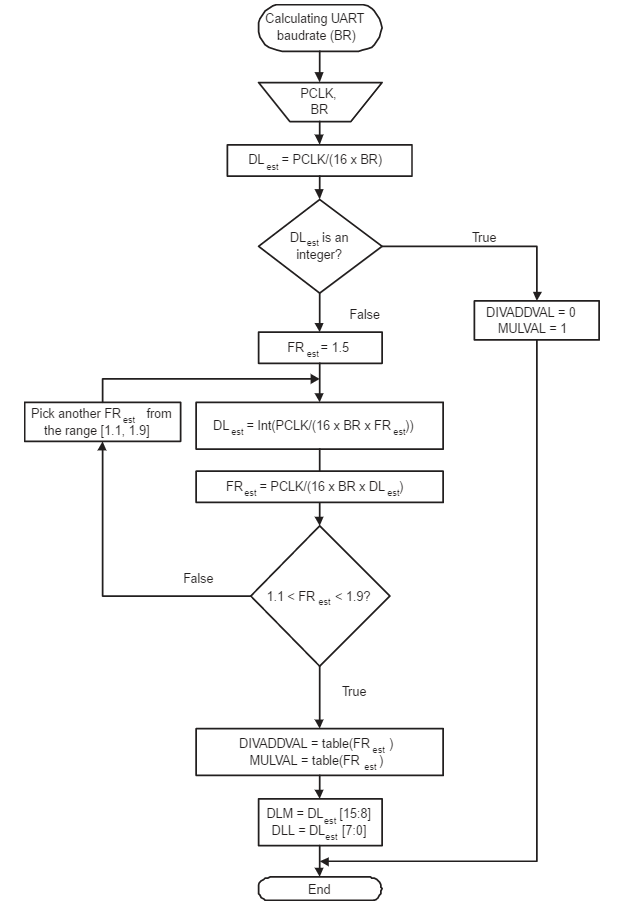
\includegraphics[scale=.85]{usart_algorithm.png}
	\caption{Algorithm to calculate required values for Serial baud rate}
	\label{fig:serial_algo}
\end{figure}

\subsubsection{Auto-Baud}

Another option to account for this is a feature provided within the processor called Auto-Baud\cite{mbed_datasheet}. This is where the device waits on receiving communication upon its RX pin and of the data coming in, it measures the baud rate between a falling edge and a subsequent rising or falling edge depending on the mode set within the registers.

Using this information, the required registers are set to enable Serial communication such that the device can communicate at the required baud rate. To enable an effective method for enabling auto baud, a python script was created which can be used on the host PC. This script continuously sends the character 'g' whilst also receiving and printing bytes. The continuous stream of 'g's gives a signal for auto baud to configure itself and should the device be reset during communication it will be configured automatically after reset should the script be running.

\subsection{Getting Sensor Data}

With \todo{Should this be moved to the I2C subsection?} the sensor libraries re-written to be compatible with the ARM libraries, the sensor can be interfaced with the mBed. Upon the sensor, all pins used were on Junction 4. This pins connected between the mBed and sensor were the data line, pins 28 and 3 respectively, as well as the clock line, pins 27 and 2 respectively. These pins were also connected to pull-up resistors with values of 2.2k\ohm. Power was also supplied to the sensor from the mBed from its 3.3V Regulated Output which went to pin 1 of the sensor along with a common ground between the Ground pin of the mBed and pin 6 of the sensor. 

Once done, it was possible to extract sensor readings from the device, depending on what data is required a variety of different functions from the library can be used.

\begin{description}
	\item[Accelerometer X axis] \hfill \\ getAccelerationX
	\item[Accelorometer Y axis] \hfill \\ getAccelerationY
	\item[Accelorometer Z axis] \hfill \\ getAccelerationZ
	\item[Accelerometer all axis] \hfill \\ getAcceleration
	\item[Gyroscope X axis] \hfill \\ getRotationX
	\item[Gyroscope Y axis] \hfill \\ getRotationY
	\item[Gyroscope Z axis] \hfill \\ getRotationZ
	\item[Gyroscope all axis] \hfill \\ getRotation
	\item[Accelerometer and Gryoscope all axis] \hfill \\ getMotion6
\end{description}

\todo{Do something about this}

Thus allowing for a variety of possibilities for obtaining data from the sensor, as should only certain data be required, a function can be chosen which reduces the amount of data being received, hence reducing the communication time between the mBed and sensor.

\subsection{Getting the desired sampling rate}

The model employed requires a set sampling rate, and to minimise the communication between the mBed and device to minimise processing, the mBed should sample the sensor at the sampling rate required by the model. To achieve this, there a few different parameters tweaked, specifically the Watchdog \verb|FCLKANA| and \verb|DIVSEL| as well as SCLL and SCLH for the I2C clock. These values represent the number of clock cycles the I2C clock remain low and high respectively, where the lowest value they may have is four. Thus, can be used to speed up or slow down I2C communication. \cite{mbed_datasheet} This can be summed in Equation~\ref{eqn:i2c_clock}.

\begin{equation}
	I2C_{clock} = \frac{CLK}{SCLH + SCLL}
	\label{eqn:i2c_clock}
\end{equation}

It was decided that the duty cycle of the I2C clock is 50\%, hence the value of SCLL and SCLH should be the same. A similar method, from when measuring the frequency of the oscillator with varying voltage via a pin, was used where the frequency of the pin is half the sampling rate. This because in one cycle of the pin, it goes through the while loop twice and the sensor is queried once each loop.

\subsection{Issues}

There were a variety of issues that were encountered with the mBed. It was possible to remedy some of the issues, however not all.

It was found that forgetting to power on the Watchdog oscillator before switching the system clock over to it left it in a state where it was unable to execute any code. This state, for unknown reasons, persisted even after a reset and reboot of the device. An eventual solution to this problem was found, which was to re-flash the mBed interface firmware.

SPI communication was attempted to interface the mBed to a SD card allowing for data from the sensor to be stored within the SD card so it is possible to revisit collected data at a later point in time. This would be especially useful should the device not be connected to the host PC to send debug information to. Navigating the mBed site does show a library with functionality perfect for this aim, however attempting to compile the example code resulted in a error during compilation due to the fact the binary would have been larger than the flash capacity of the mBed. Switching over to the online compiler provided by mBed resulted in compilation however the binary would not execute upon the mBed.

An issue occurred when optimising multiple multiplication and division operations into a single bit shift however, the output of said optimisation caused the code to return different results compared against the unoptimised version upon the mBed however not on another machine. This was found to be due to the fact that the mBed stores its variables in a little endian format.

\subsection{Measuring power}

It is required to measure the power of the system as a requirement is for it to be low powered as the sub threshold processor will be operating at a low power. It was deemed unnecessary to measure the power consumption of the mBed because of the various peripherals which are also powered which would not be there on the sub threshold version as well as the fact that this processor is not designed for sub threshold power and the method ARM implement to achieve this may leave a different power fingerprint than the Cortex M0. 

The sensor however does not fall under the same conditions and thus, was analysed for its power usage. To do this a 100\ohm ~resistor was placed in series between the sensor and $V_{cc}$. Thus current would have to flow through the resistor to reach the sensor, allowing to measure the current by measuring the voltage across the resistor along with the relationship V=IR.

The power consumption of the sensor is not constant over time due to the fact that the sensor alternates between sleep mode and being awake. It also will consume more power when communicating over I2C as opposed to not. To account for this, the current and voltage is measured over time which is then averaged thus, giving the average power consumed by the sensor.

\begin{table}
	\centering
	\begin{tabular}{|l|r|r|}
		\hline
		Parameter & Mean Value & Standard Deviation \\
		\hline
		Resistor Voltage (V) & 0.0262 & 0.00198 \\
		Sensor Voltage (V) & 3.29 & 0.00133 \\
		Current (A) & 0.000262 & \\
		Power (W) & 0.00086198 & \\
		\hline
	\end{tabular}
	\caption{Power statistics for the sensor}
	\label{tab:power}
\end{table}

As can be seen from Table~\ref{tab:power}, the sensor on average took $861\mu W$ which can be considered low power. However, there is the potential for a lower power consumption, within the configuration used, the current flowing through the sensor was $262\mu A$, but the data sheet for the sensor says for the sampling rate and configuration that is being used, the typical value is $70\mu A$. This decrease would reduce the power consumption by over a factor of 3 leaving a power usage of $230\mu W$.

\subsection{Prototyping}

During development, breadboard was used to prototype the system with both the mBed and sensor placed upon. The power rails on the breadboard received power from the mBed which in turn received power from the host PC via USB. These conditions were acceptable when developing, however was impractical for moving the device to the foot for further testing. 

It was decided to create a small board for this purpose using veroboard which would be powered with a few AA batteries. This is beneficial as the board can be made to a desired size with on-board power alleviating the requirement of having a cable trailing to a computer as well as being more comfortable on the foot over the breadboard.

A design was created using fritzing \cite{fritzing} which can be seen in Figure~\ref{fig:veroboard_schematic}. The mBed has a $V_{in}$ pin upon pin 2 which can take from 4.5V up to 9V which is supplied using four AA batteries within two AA battery holders. To prevent the mBed from constantly being powered, a jumper is added to control whether the mBed receives power or not enabling for the device to be switched on or off at will. Power to the sensor is provided via the 3.3V regulated output of the mBed, which also is used by the pull-up resistors to hold the I2C lines high when not in use. Extra space was added above and below the sensor due to the fact that the physical board is larger than that in the CAD software upon that axis, thus requires more space to avoid colliding with the mBed or hanging off the edge of board.

\begin{figure}
	\centering
	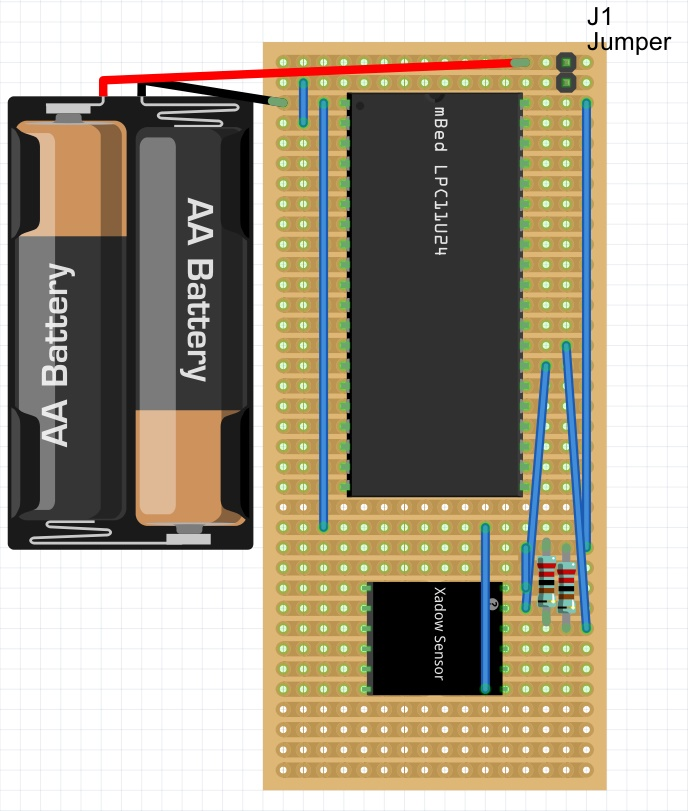
\includegraphics[scale=.6]{veroboard_schematic.png}
	\caption{Schematic for veroboard}
	\label{fig:veroboard_schematic}
\end{figure}

This was then built, as can be seen from Figure~\ref{fig:board}. To avoid having to solder on the actual mBed and sensor to the veroboard, female header pins are used in a manner similar to IC holders allowing for them to be placed and removed from the board as required. For compactness, the battery packs were attached to the underside of the board using velcro. 

\begin{figure}
	\centering
	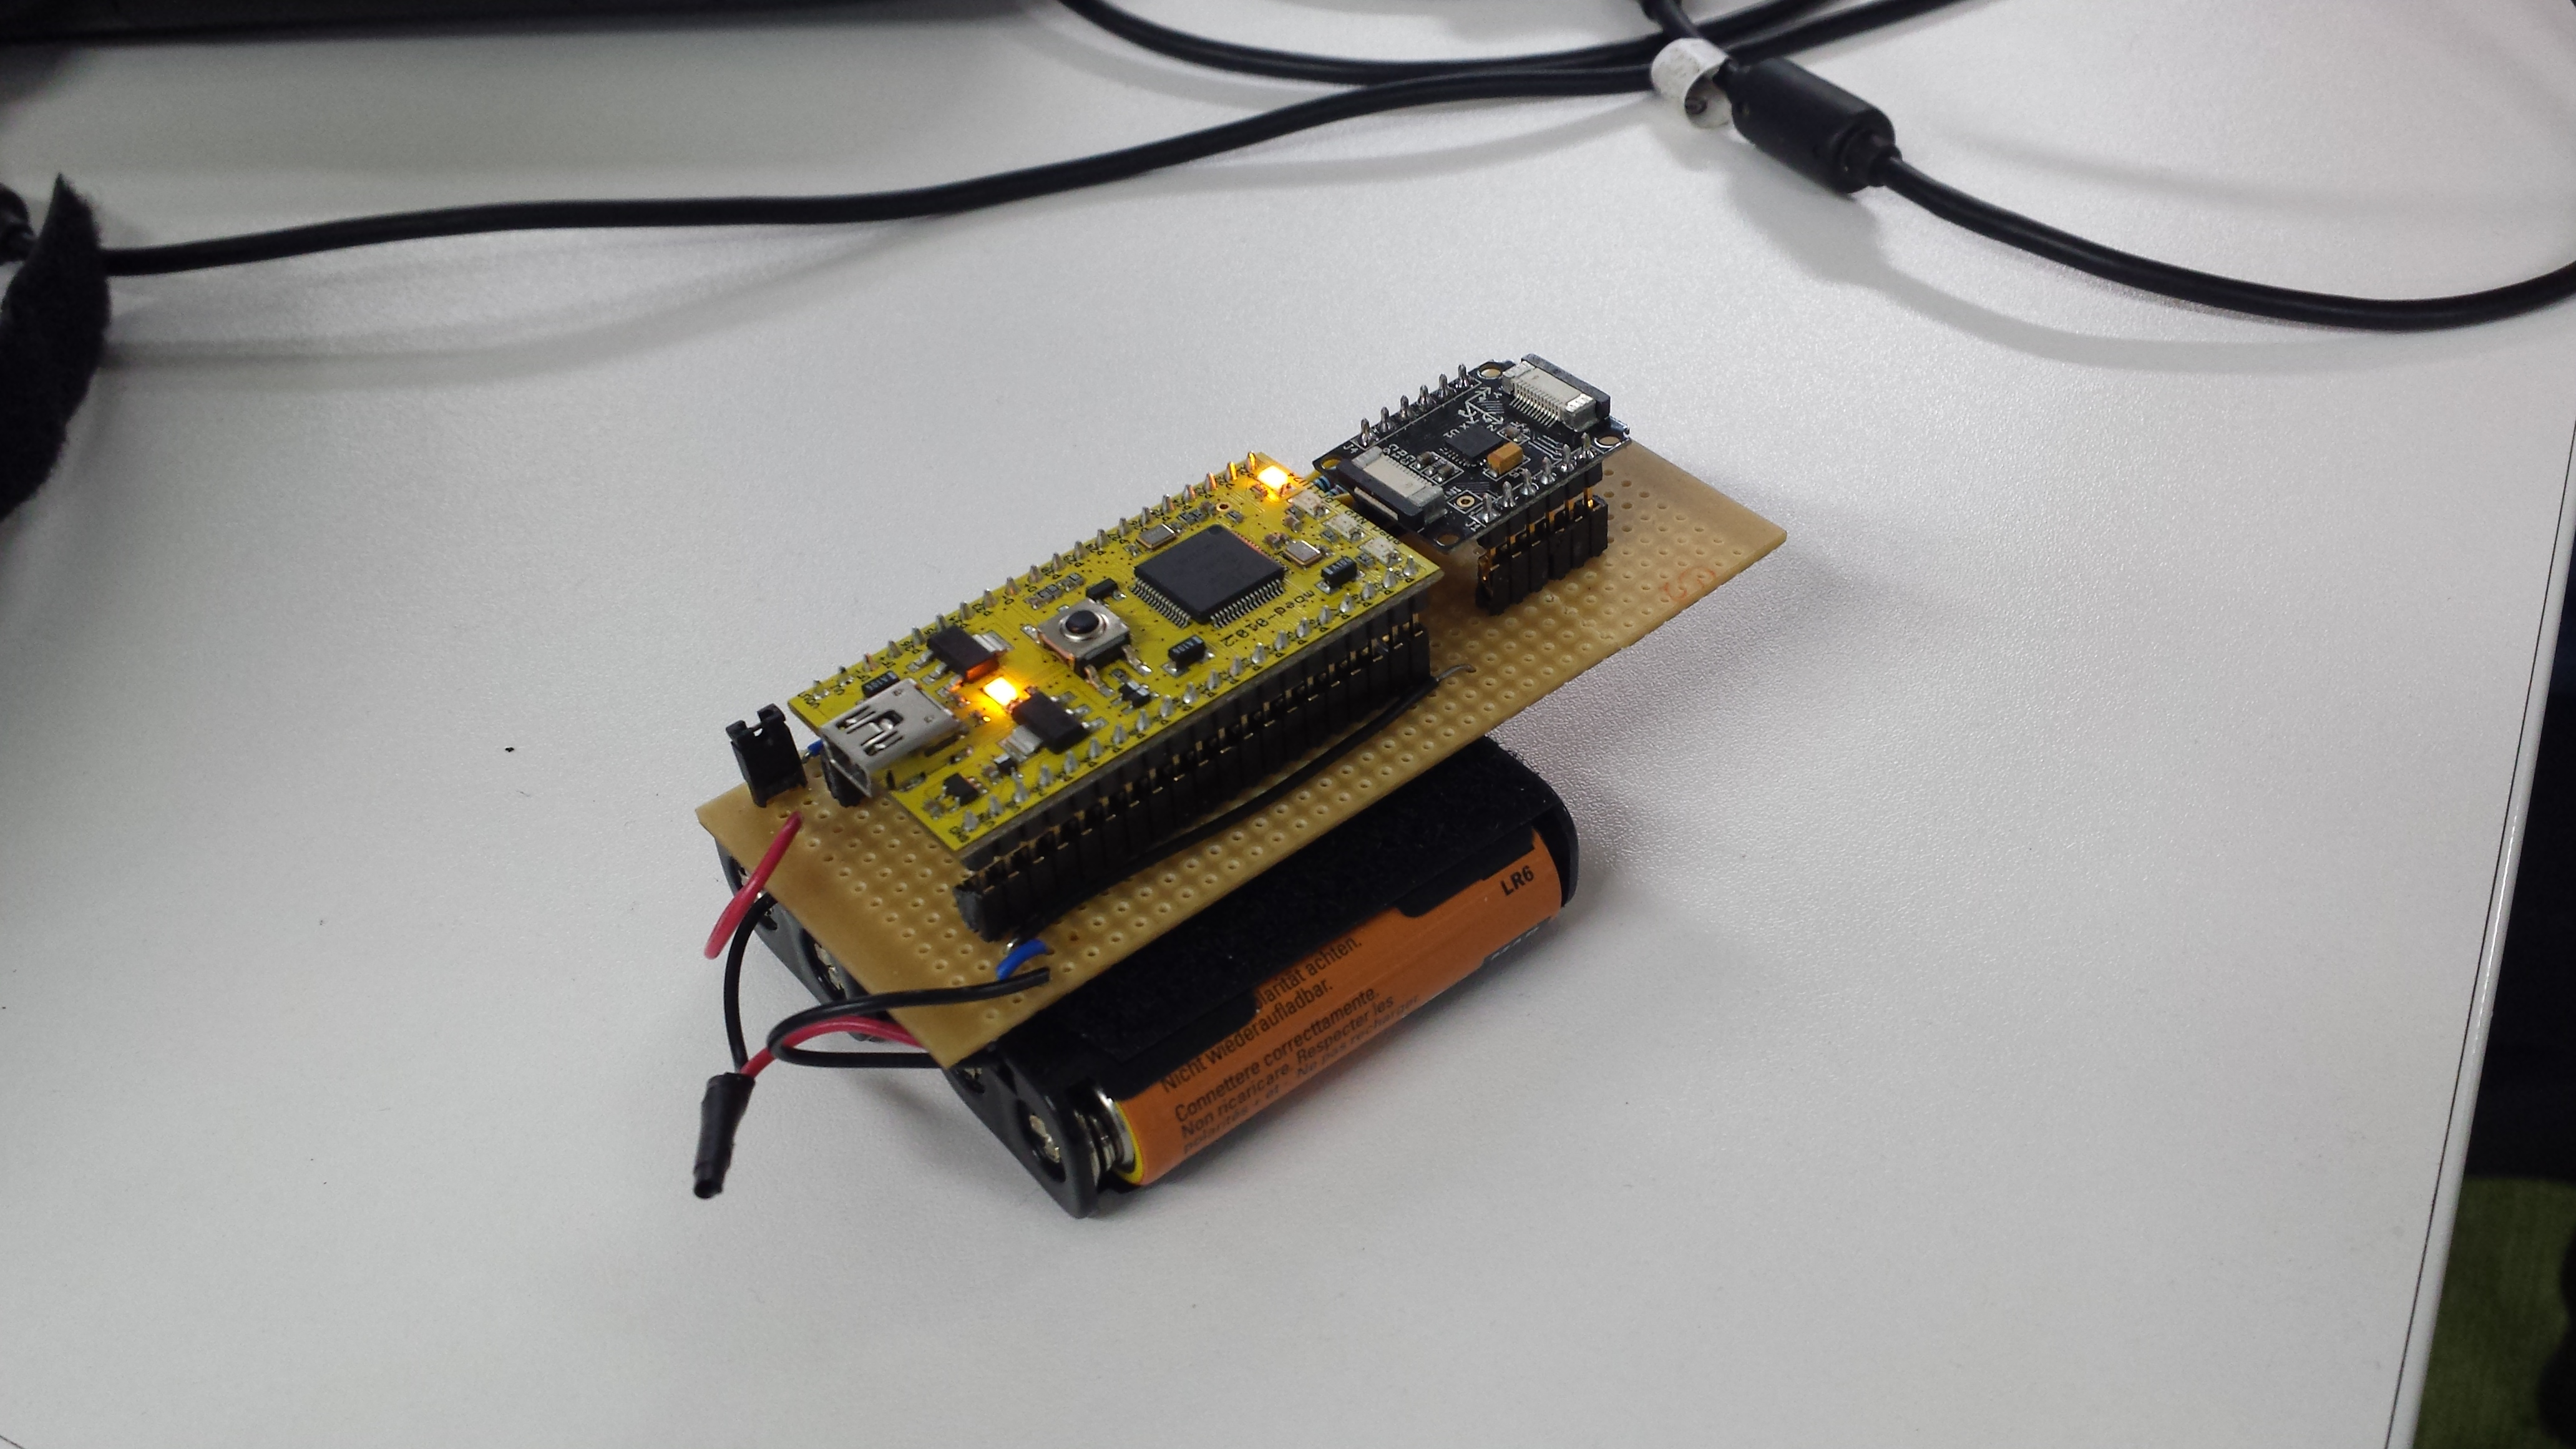
\includegraphics[scale=.1]{prototype_no_straps.jpg}
	\caption{Prototype board}
	\label{fig:board}
\end{figure}

The board was now able to be placed upon a foot, however there was nothing to secure it in place. A similar approach was taken from the participant study of using velcro. Two pieces of velcro would be attached to the board, whilst another two to the foot. This would then allow the board to be placed on the foot with the velcro holding the board onto the foot. The reasoning for using two pieces of velcro over one is that it was found to allow for more stability when on the foot over one piece where it leaves room for the board to start rotating forwards and backwards. The board with the velcro can be seen in Figure~\ref{fig:board:velcro}.

\begin{figure}
	\centering
	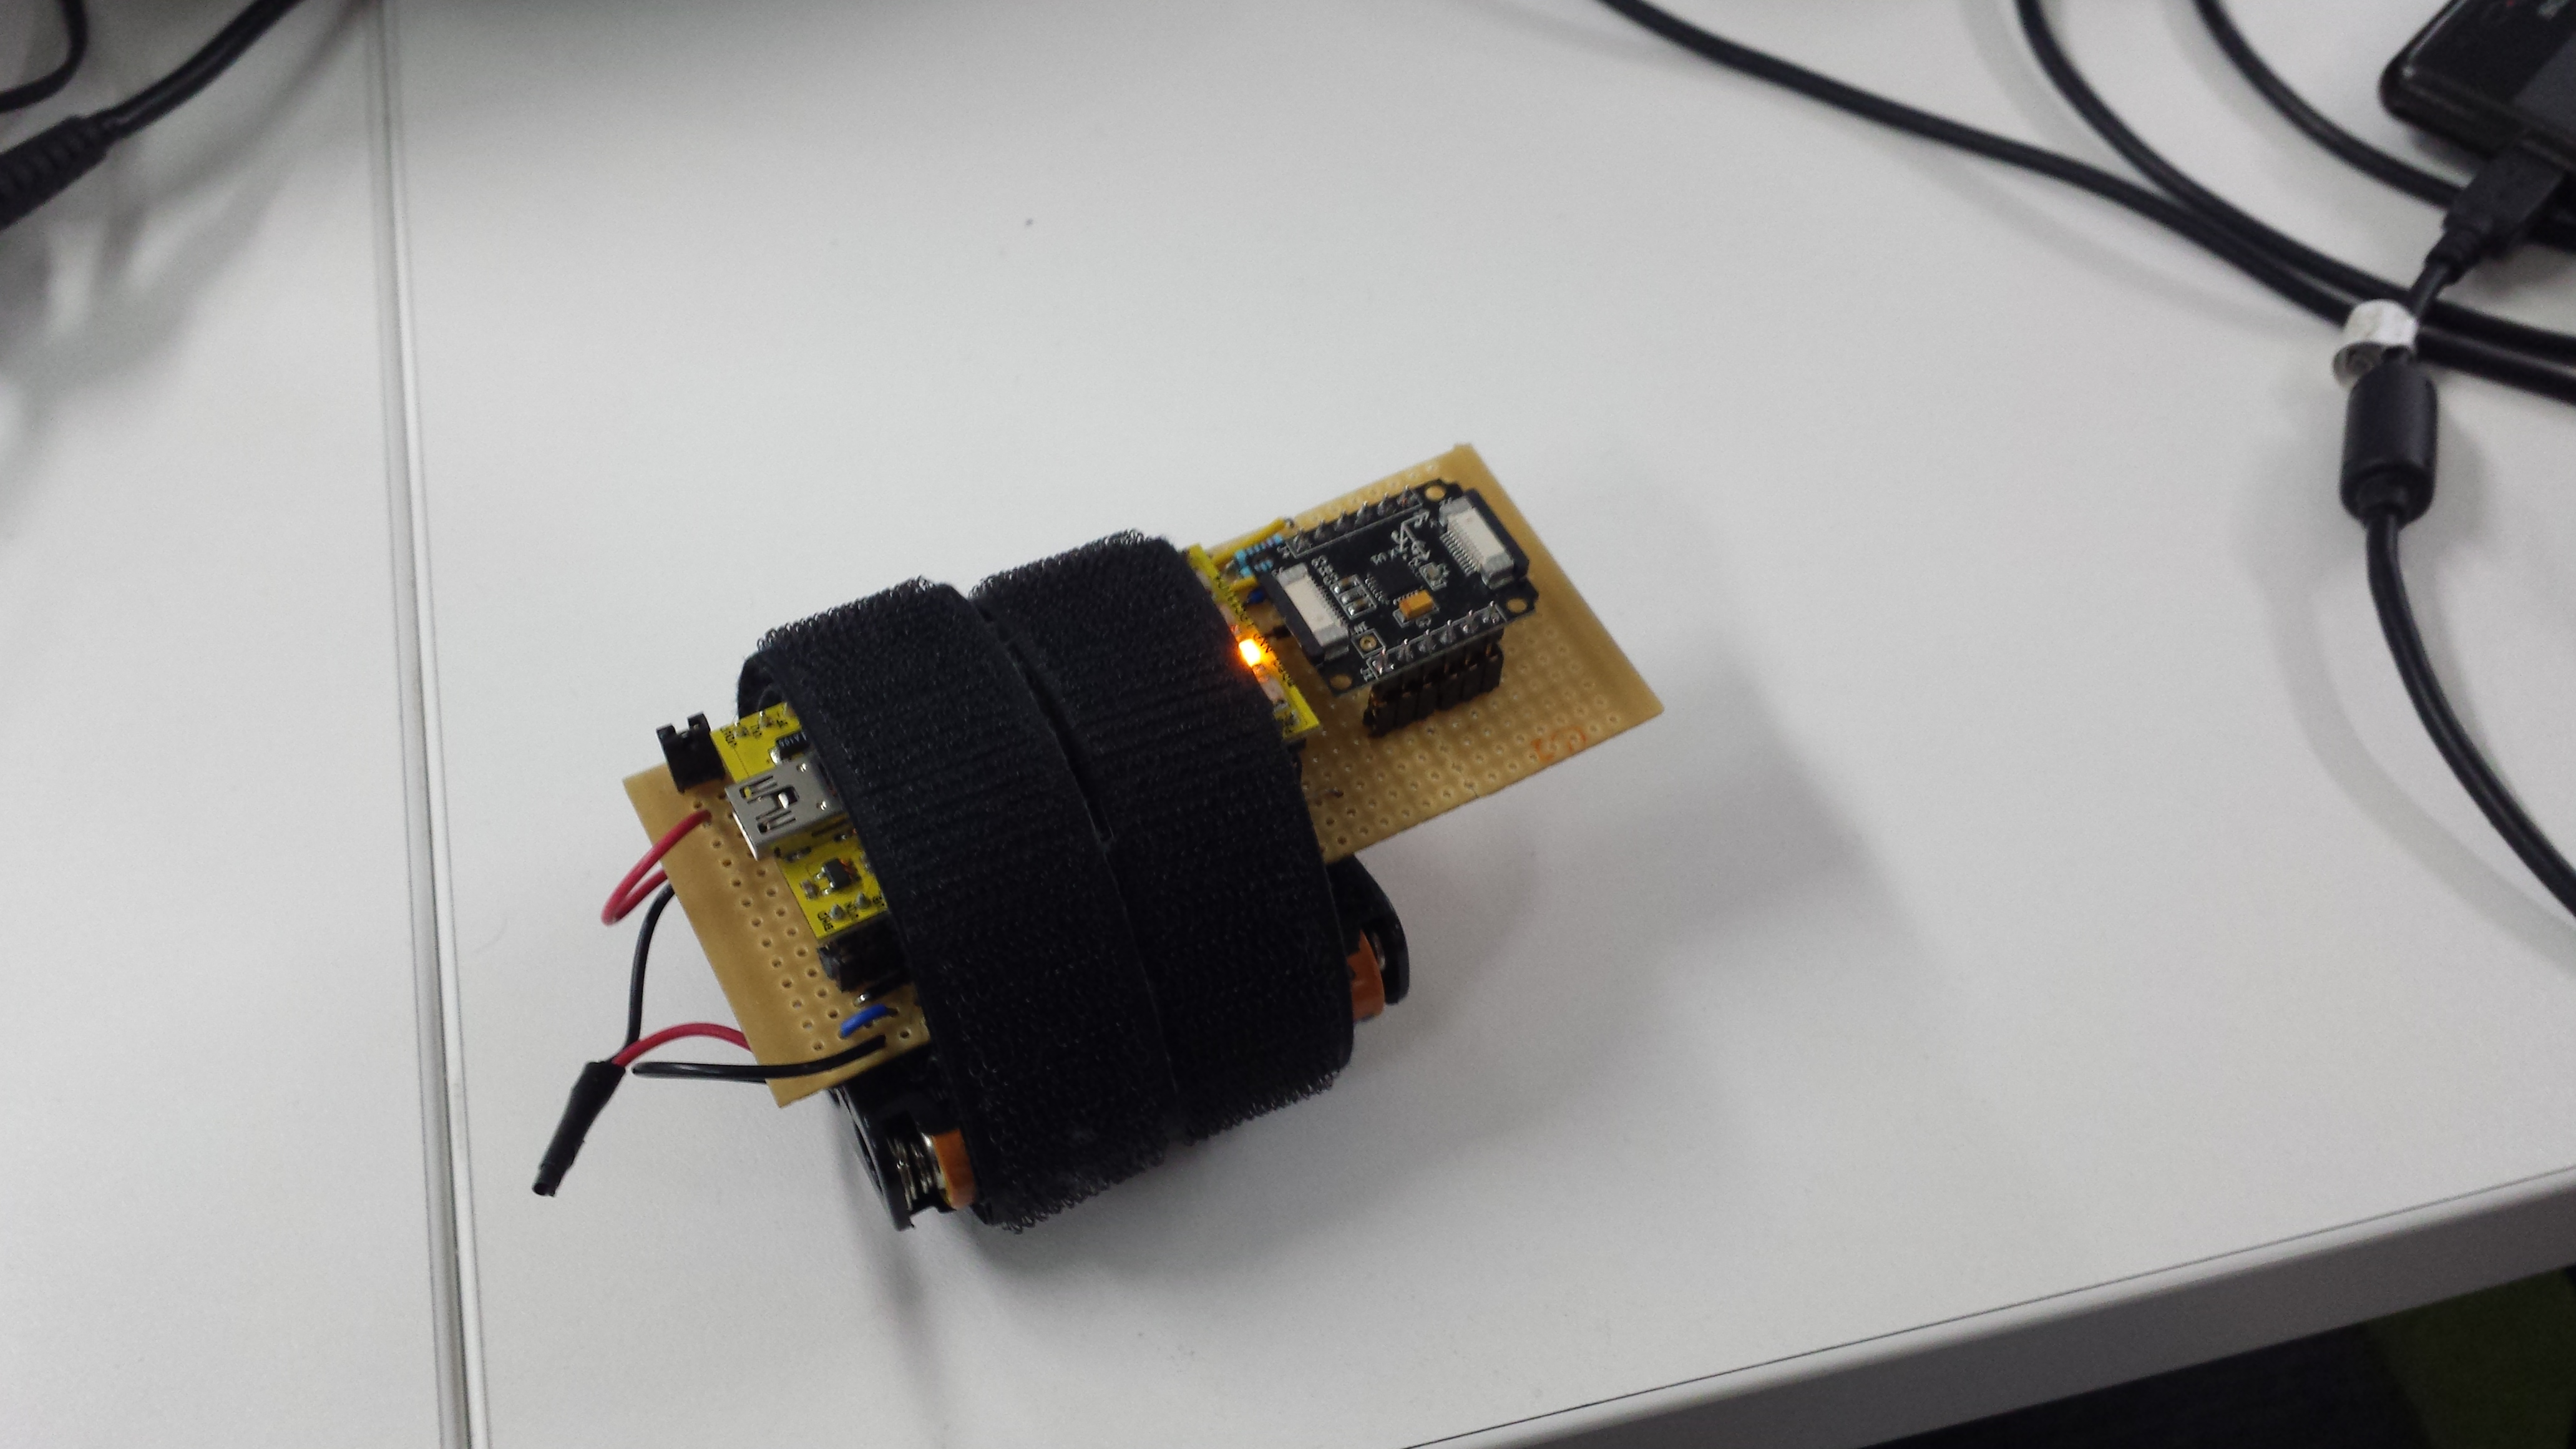
\includegraphics[scale=.1]{prototype_straps.jpg}
	\caption{Prototype board with velcro straps}
	\label{fig:board:velcro}
\end{figure}
\namedsection{Final Design}{Gupta}

The final layout of the hardware does indeed follow what was initially planned. As can be seen from Figures~\ref{fig:hardware_schematic_development-2} and~\ref{fig:hardware_schematic_final-2} as compared to Figures~\ref{fig:hardware_schematic_development} and~\ref{fig:hardware_schematic_final}, they are pretty much the same diagram except the actual protocols for communication are ironed out. 

The LED for the mBed was straightforward to do and did not require any additional hardware due to the fact that the mBed has four user programmable LEDs on board allowing for the desired visual output as well as a few additional for an extra level of debugging, especially when the device is not connected to the host PC via the serial connection.

\begin{figure}
	\centering
	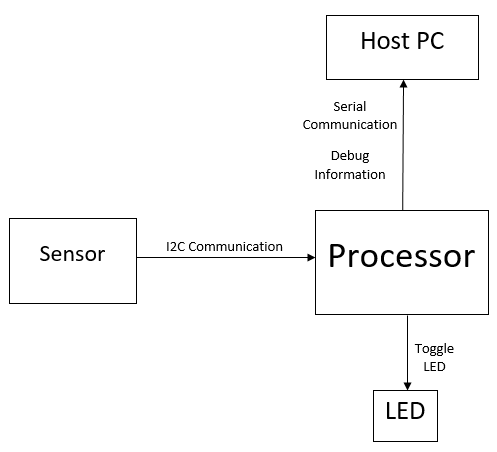
\includegraphics{hardware-schematics-development-2.pdf}
	\caption{Final Hardware Block Diagram - Development}
	\label{fig:hardware_schematic_development-2}
\end{figure}

\begin{figure}
	\centering
	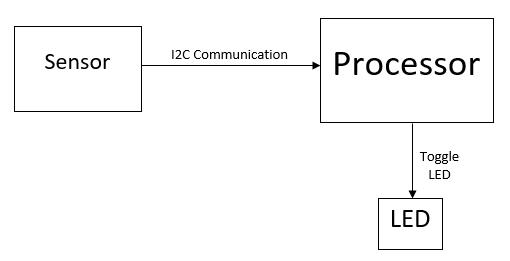
\includegraphics{hardware-schematics-final-2.pdf}
	\caption{Final Hardware Block Diagram - Final}
	\label{fig:hardware_schematic_final-2}
\end{figure}